\section{Tidal streams}\label{sec:streams}

Tidal streams are the application for which \galpy's DFs are most often
fit to data, and the one in which derivatives have been most sorely
missed, because a stream model is an expensive forward computation with
a handful of parameters, the potential's among them, and fitting it has
meant exploring that parameter space with a sampler that knows nothing
of the model's smoothness. \galpy\ contains three stream models, all of
which now run on the backends: the action--angle model of
\citet{Bovy2014}, \texttt{streamdf}, with its extension to stream gaps
\citep{Sanders2016}; and the particle-spray models of \citet{Fardal2015}
and \citet{Chen2025}, \texttt{streamspraydf}.

\subsection{The action--angle stream model}\label{sec:streams-streamdf}

\texttt{streamdf} models a stream as a distribution in frequency and
angle space, computes the mean track of the stream in configuration
space by iterating the transformation between the two, and samples and
evaluates the DF around that track. On the backends the track
computation is a pure function of the progenitor's orbit and the
potential that is vectorized over the segments of the track and is
differentiable from end to end: the auxiliary orbits are integrated in
the backend, and the Jacobian of the action--angle transformation along
the track, which was a finite-difference Jacobian in the \numpy\ code,
is the automatic Jacobian of the methods of \sectionname~\ref{sec:aa}.
The derivative of the track with respect to a parameter of the
potential agrees with a finite difference of the same computation to a
few parts in $10^4$, which is the level set by the fixed iteration count
of the track refinement. Construction of a \texttt{streamdf} is
differentiable with respect to the potential, and can be compiled,
although the compilation of a construction, which contains tens of
orbit integrations and the iteration of the track, takes a quarter of an
hour and is only worthwhile when many streams are to be built; the
construction itself, once compiled, takes about a minute on a CPU,
compared with a few to tens of seconds for the \numpy\ and \cc\ version.
Sampling and evaluating the DF, on the other hand, are two orders of
magnitude faster under compilation than on \numpy, and run on a GPU.

A point about these derivatives is general enough to state here. A
stream model is a generative model: the stream's stars are a sample from
the model's DF. The derivative of the track with respect to a parameter
can be taken with the sample of stars held fixed, which is what one
obtains by differentiating the track code alone, or by letting the
sample move with the parameter, which is what a finite difference of the
full model computes. The first is not a physical quantity, and the two
differ. Where \galpy\ provides derivatives of stream models, they are of
the second kind, and they are tested against finite differences whose
step is shown to be converged.

\subsection{Particle-spray models}\label{sec:streams-spray}

The particle-spray models release particles from the progenitor at
random times with random offsets in position and velocity and integrate
them forward. On the backends, \texttt{sample()} and the track-fitting
method \texttt{streamTrack()} are pure functions of the progenitor's
orbit, the potential, the progenitor mass (or a mass history), and a
random key: the stripping times are drawn by inverse transformation of
uniform variates, the offsets by reparameterized normal variates, the
progenitor and the particles are integrated in the backend, and the
track is fit with a penalized spline. The whole computation compiles
and is differentiable with respect to every parameter,
\begin{code}
key= galpy.backend.random.key(1,backend='jax')
def leading_arm(q):
    spdf= fardal15spraydf(mass,progenitor=Orbit(ic),tdisrupt=4.5/time_in_Gyr(),
                          pot=LogarithmicHaloPotential(normalize=1.,q=q))
    return spdf.sample(n=1500,return_orbit=False,tail='leading',key=key)
track_and_dtrack= jax.jvp(leading_arm,(q0,),(1.,))
\end{code}
where the forward-mode derivative gives the change of every particle's
position for a unit change in the halo flattening, with the random
numbers in common between the two. The derivative of the sampled stream
with respect to the potential agrees with finite differences of the same
sample to $10^{-6}$, and \figurename~\ref{fig:extrapolation}
demonstrates what it is good for: a single pass of forward-mode
differentiation over a 1500-particle stream predicts the stream's track
in a halo of different flattening well enough to remove most of the
shift in the track for changes in the flattening of up to twenty
percent, which is the kind of step a fitter takes. Each spray
particle's orbit is one more orbit in a batch, such that a sprayed
stream costs about a millisecond per particle on a CPU under compiled
\jax, about half the cost of the non-differentiable \cc\ version, and
microseconds per particle on a GPU (\figurename~\ref{fig:spraysp}).

\begin{figure}[t!]
  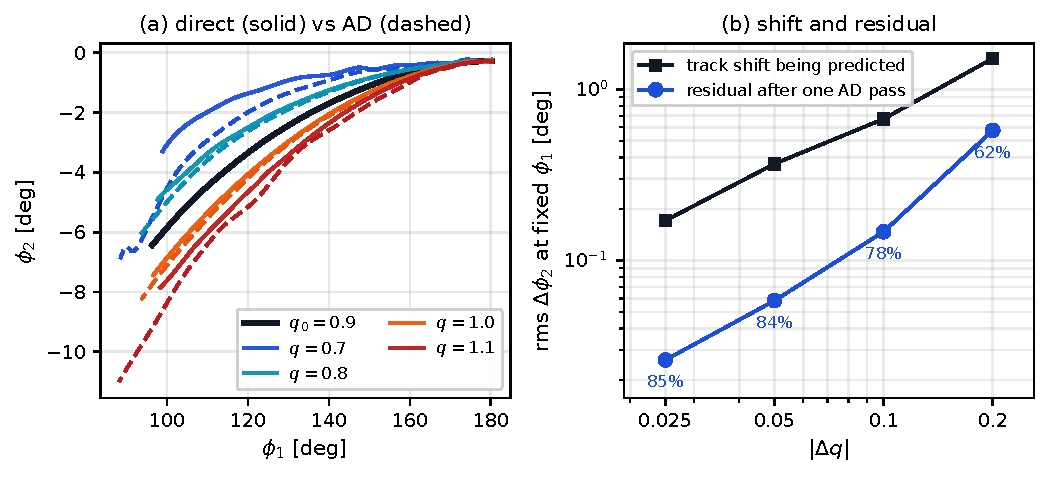
\includegraphics[width=0.48\textwidth,clip=]{../figures/gS3_track_extrapolation/gS3_track_extrapolation.pdf}
  \caption{Predicting a stream's track in a different potential from one
    derivative. Left: the track of a 1500-particle \texttt{fardal15spraydf}
    stream after 4.5\,Gyr in a logarithmic halo with flattening
    $q_0=0.9$ (black), the tracks in halos with $q=0.7$ to $1.1$
    computed directly (solid), and their prediction from the forward-mode
    derivative of the stream with respect to $q$ at $q_0$ (dashed), in a
    coordinate frame aligned with the progenitor's orbit. Right: the
    root-mean-square shift of the track at fixed $\phi_1$ and the
    residual after the first-order prediction, as a function of
    $|\Delta q|$.}\label{fig:extrapolation}
\end{figure}

\begin{figure*}[t!]
  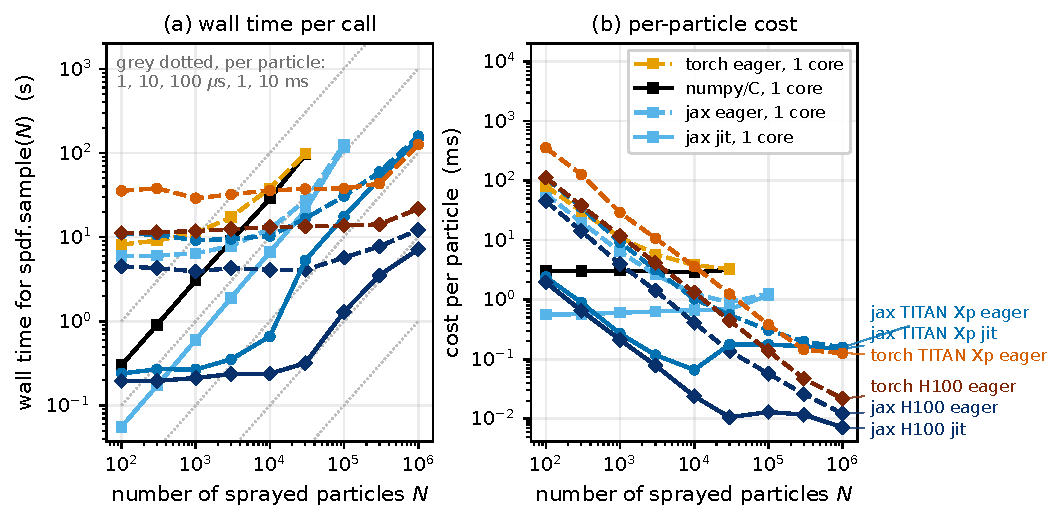
\includegraphics[width=\textwidth,clip=]{../figures/gS5_streamspray_speed/gS5_streamspray_speed.pdf}
  \caption{Speed of the particle-spray stream model: wall time (left)
    and cost per particle (right) of \texttt{fardal15spraydf.sample(N)}
    with 4.5\,Gyr of stripping, for the \numpy\ version with the \cc\
    integrator and for the differentiable backend version on the CPU,
    the TITAN~Xp, and the H100, compiled (solid) and eager
    (dashed).}\label{fig:spraysp}
\end{figure*}

\subsection{Stream gaps}\label{sec:streams-gaps}

The stream-gap model of \citet{Sanders2016}, \texttt{streamgapdf},
computes the velocity kick that a passing subhalo imparts along a stream
and propagates it through the action--angle model. The kick kernels for
the Plummer and Hernquist subhalos, the interpolation of the kicks along
the stream, and the transformation to the impact frame run on the
backends and are differentiable with respect to the parameters of the
impact, and the orbit integrations in the model go through the batched
in-backend solver when given backend inputs. The construction of the
model is not traceable, because it assigns into arrays in place in
many places, and this was left as it is.
